% Submission copy for SPLASH 2026 Onward! Essays (single-blind).
% Built from paper/main.tex at the same commit; venue-specific changes:
%   - acmart sigconf template instead of article 12pt
%   - explicit single-blind author identification (heznpc)
%   - Zenodo deposit citation removed for first-round submission
%     (per submissions/onward-essays-2026/anonymization-notes.md; can be
%      restored at camera-ready time)
\documentclass[sigconf, nonacm, anonymous=false]{acmart}

\usepackage{amsmath}
\usepackage{booktabs}
\usepackage{url}
\usepackage{array}
\usepackage{tabularx}
\usepackage{tikz}

% acmart loads hyperref and natbib; keep hyperref colors visible for review PDF
\hypersetup{
  colorlinks=true,
  linkcolor=blue,
  citecolor=blue,
  urlcolor=blue
}

% Suppress conference / DOI / ISBN preprint placeholders (Onward! Essays
% review version, not yet a camera-ready artifact)
\settopmatter{printacmref=false}
\renewcommand\footnotetextcopyrightpermission[1]{}
\pagestyle{plain}

\title{The Metadatafication of Version Control: How AI Agents Transform Git from Tool to Infrastructure}

\author{heznpc}
\affiliation{%
  \institution{Independent}
  \country{Korea}
}
\email{heznpc@gmail.com}

\begin{document}

% acmart renders the title block (title, authors, affiliations, abstract)
% only when \maketitle is invoked. The abstract environment must be
% declared BEFORE \maketitle so it appears in the title block.
\begin{abstract}
We document five concurrent failure modes of agent-era Git workflow---unpushed commits, stale worktrees from merged pull requests, silent partial failure of \texttt{gh pr merge --delete-branch}, external-contributor issues that never reach the agent, and IDE-resident session lifecycle drift---and argue they instantiate one mechanism: \textit{metadatafication}, the transition of an operator-driven tool into automatically-generated infrastructure metadata. Drawing on Star and Ruhleder's claim that mature infrastructure becomes visible only upon breakdown, we propose three measurable quantities---Agent-Push Latency (APL), Metadata-Invisibility Period (MIP), Push-Leakage Rate (PLR)---and a fourth (Uncommitted-Period, UCP) for the analogous working-tree layer, and we deploy them as a portable instrument on one operator's 57-repository portfolio. The single-operator case study illustrates the instrument's discrimination power; the instrument itself is what the artifact contributes, with the case study as worked example rather than population claim. We position the resulting Canary MCP server as a layer of \textit{agent-readable observability} distinct from the cloud-side workflow tooling (GitHub Agentic Workflows) entering preview during the same window, and we identify the operator-machine surface as the gh-aw-uncopable zone where the metadatafication thesis is most empirically tractable. The community that adapts will treat agent-readability---not human-readability---as the primary design target for the records its tools generate.
\end{abstract}

\maketitle

\section{Introduction}

In April 2005, Linus Torvalds released the first version of Git to manage Linux kernel development. In the two decades since, Git has become the de facto standard for version control, with GitHub alone hosting over 420 million repositories as of 2025. During the same twenty-year span, the technology industry witnessed multiple paradigm-level disruptions: Yahoo's curated directory gave way to Google's algorithmic search, Blockbuster's physical rental model collapsed under Netflix's streaming, and the music industry's \$14 billion CD economy imploded before reconstituting around streaming platforms \citep{mindsetai2026saas}. Each transition followed a recognizable pattern: the underlying need persisted, but the interface through which users interacted with it was radically restructured.

We argue that version control is now entering a similar transition. The trigger is not a new version control system, but a new class of user: AI coding agents. Empirical evidence shows that AI agents are already significant contributors to open-source development. \citet{li2025rise} document over 456,000 pull requests authored by five leading agents (OpenAI Codex, Devin, GitHub Copilot, Cursor, and Claude Code) across 61,000 repositories. \citet{ogenrwot2026how} find that agentic pull requests differ substantially from human-authored ones in commit patterns and description-to-diff similarity. The JetBrains 2026 developer survey reports that 73\% of engineering teams now use AI coding tools daily, up from 18\% in 2024.

The prevailing discourse frames this shift as a binary: Git is either dying or it is fine. We reject both positions. Instead, we introduce the concept of \textit{metadatafication}---the process by which a directly-operated tool transitions into automatically-generated background data that persists but is no longer directly manipulated by its end users. Git's commit history, branches, and diffs will continue to exist, much as EXIF metadata exists on every photograph. But the developer who directly runs \texttt{git add}, \texttt{git commit}, and \texttt{git push} will become as rare as the photographer who manually records ISO settings on a notepad.

This paper makes four contributions, ordered by what is most directly verifiable:

\begin{enumerate}
  \item \textbf{A pattern.} We document five concurrent failure modes in agent-era Git workflow that, on inspection, instantiate one operator--tool breakdown mechanism: push-leakage, worktree-leakage, command-cleanup-leakage, contributor-issue-leakage, and IDE-session-leakage. Each is corroborated by independent external evidence (Section~\ref{sec:vignette}) ranging from open issues in the GitHub CLI tracker to public reports in the Claude Code project itself. The pattern's existence does not require the empirical study below; the study quantifies the mechanism.
  \item \textbf{An instrument.} We propose three measurable quantities, deployable on any operator's machine: Agent-Push Latency (APL), Metadata-Invisibility Period (MIP), and Push-Leakage Rate (PLR), plus a fourth (Uncommitted-Period, UCP) for the working-tree layer. The metric definitions are tooling-agnostic and reproducible; we provide a reference implementation but the metrics outlive any single codebase.
  \item \textbf{A worked case.} We deploy the instrument on one operator's 57-repository portfolio. The case study illustrates the instrument's discrimination power (it identifies a 23-of-57 leakage cluster within a 3-hour MIP window---a signature of bulk operator behaviour rather than independent slippage) without claiming population-scale generality; we are explicit (\S\ref{sec:tov}) that the case demonstrates the instrument, not the prevalence.
  \item \textbf{An architectural position.} We frame agent-readable observability as a distinct layer from the cloud-side workflow tooling that entered technical preview in the same window (GitHub Agentic Workflows, 2026-02). The two are composable rather than competing: server-side workflow tooling owns the GitHub-API-visible surface; operator-machine observability owns the local-git-and-session-transcript surface that server-side tools cannot, by construction, reach. The metadatafication thesis is most empirically tractable in the latter.
\end{enumerate}

Earlier framings of related ideas exist---\citet{star1996steps} on infrastructure visibility-upon-breakdown, \citet{li2025rise} on 456k agent-authored PRs as a macro-scale corpus, \citet{pinera2026rethinking} on sessions replacing branches---and we draw on each, but the specific synthesis of five-instance pattern + measurable instrument + architectural position is, to the best of our knowledge, new.

\section{Background and Related Work}

\subsection{Infrastructure Studies}

The idea that technologies become invisible as they mature has deep roots in science and technology studies (STS). \citet{star1996steps} identified eight dimensions of infrastructure, including \textit{transparency} (``it does not have to be reinvented each time'') and \textit{learned as part of membership} (``strangers and outsiders encounter infrastructure as a target object to be learned about''). \citet{edwards2003infrastructure} traced how sociotechnical systems evolve from artisanal operation to automated background processes, with human expertise progressively encoded into the infrastructure itself. \citet{bowker1999sorting} showed how classification systems and their metadata become ``naturalized''---accepted as given rather than designed. We draw on this tradition to frame Git's trajectory, while introducing ``metadatafication'' as a specific mechanism within the broader phenomenon of infrastructure transparency (Section~3).

\subsection{The Agentic Turn in Software Engineering}

\citet{hassan2025agentic} propose recognizing a fundamental duality in software engineering: ``SE for Humans'' and ``SE for Agents,'' arguing that the field must radically reimagine its foundational pillars---actors, processes, tools, and artifacts. This framework, termed SE 3.0, extends beyond the AI-augmented development of SE 2.0 (copilots and code completion) into a regime where agents autonomously plan, execute, and iterate on software tasks.

The empirical reality of SE 3.0 is documented by \citet{li2025rise}, whose AIDev dataset spans 456,000+ pull requests across 61,000 repositories. Complementary studies examine the adoption patterns of coding agents on GitHub \citep{agentic2026adoption}, the barriers to merging agent-authored pull requests \citep{agentpr2026unmerged}, and the emergence of AGENTS.md files as version-controlled agent configuration artifacts \citep{agentsmd2026impact}. A growing body of work specifically examines these context files: \citet{chatlatanagulchai2025agentreadmes} analyze 2,303 context files from 1,925 repositories, finding that developers prioritize functional context (build commands, implementation details) over non-functional requirements; \citet{mohsenimofidi2025contextengineering} study 466 projects and find no established content structure, indicating the convention is still emergent; and \citet{galster2026configuring} explore structured configuration schemas as alternatives to free-form markdown. Critically, \citet{gloaguen2026evaluatingagentsmd} find that LLM-generated context files can \textit{reduce} task success rates while increasing inference costs---a finding we address in Section~7.

\subsection{Rethinking Version Control}

\citet{pinera2026rethinking} argues that Git's 2005 design assumes ``humans writing code in isolation, occasionally syncing their work---an assumption that is breaking down.'' He proposes replacing branches with \textit{sessions} that capture prompts, reasoning, code, and tests as unified contribution units, and replacing pull requests with \textit{prompt requests} where contributors submit intent rather than implementation.

The All Things Open editorial \citep{ato2026versioncontrol} highlights the scalability crisis: ``When a thousand engineers each spin up a hundred AI agents, the merge request model fails.'' They point to Atomic \citep{atomic2026}, a new VCS designed from inception for agentic workflows, as evidence that the design space is being actively explored. \citet{cohen2026manyana} proposes Manyana, a CRDT-based VCS where merges always succeed by definition, eliminating traditional conflict resolution---a design that implicitly acknowledges that human-mediated merge conflicts become untenable at machine speed.

\subsection{Spec-Driven Development and Disposable Code}

A parallel discourse argues that code itself is becoming a derived artifact. \citet{welch2025disposable} positions specifications as the ``actual source'' and code as the ``compiled binary.'' Research on the NL-code interface extends this vision architecturally: if representation-level execution becomes practical, programming languages shift from human-writable specifications to machine-generated projections---``languages become output formats'' rather than authoring tools~\citep{zgap2026chomsky}. \citet{piskala2026sdd} defines three levels of specification rigor---spec-first, spec-anchored, and spec-as-source---with the latter treating code as entirely generated and verified against specifications. GitHub's own Spec Kit \citep{github2025speckit} operationalizes this vision, and \citet{stoica2024specifications} from UC Berkeley argue that specifications are ``the missing link'' for reliable LLM systems.

The logical endpoint is \textit{ephemeral software} \citep{ellis2025ephemeral, houston2025ephemeral, ali2025ephemeral}: applications generated on demand, used briefly, and discarded. \citet{harel2025disposable} draws parallels to disposable content in social media: ``once the barrier to build collapses, usage patterns evolve.'' The JIT Coding framework \citep{playbooks2025jit} articulates this as ``the spec is the program, code is just exhaust.''

\subsection{The One-Person Company Hypothesis}

Anthropic CEO Dario Amodei has stated with ``70--80\% confidence'' that the first billion-dollar single-employee company could appear in 2026 \citep{nxcode2026unicorn}. This is not merely a prediction about productivity tools but a structural claim about the firm: if AI agents can perform the work of an engineering team, the organizational rationale for multi-person software companies weakens. The effect may be multiplicative: non-English-speaking developers currently face a double translation (native thought $\to$ English syntax $\to$ execution), and research on reasoning-language effects suggests this overhead is substantial~\citep{li2026reasoning}. Representation-level systems could eliminate this double translation~\citep{zgap2026chomsky}, expanding the global talent pool and further enabling the solo-founder model.

\section{The Metadatafication Thesis}

\subsection{Definition}

Our concept of metadatafication builds on a rich tradition in infrastructure studies. \citet{star1996steps} established the foundational insight that infrastructure becomes visible only upon breakdown: mature infrastructure is characterized by ``transparency''---it is ``invisibly [supporting] tasks'' without requiring active attention. \citet{edwards2003infrastructure} extended this to show how sociotechnical systems embed human knowledge into automated processes over time, with the original human expertise becoming ``black-boxed'' within the infrastructure. \citet{bowker1999sorting} further demonstrated how classification systems---including the metadata they generate---become invisible as they mature, shaping practice without being noticed.

Metadatafication describes a specific trajectory within this broader pattern: the transition from direct tool operation to automatic metadata generation, where the tool's \textit{outputs} persist but the \textit{interaction} disappears. This is narrower than Star and Ruhleder's ``infrastructure transparency,'' which encompasses all forms of background operation. The distinction matters because metadatafication makes a stronger empirical claim: not merely that the tool fades from attention, but that its outputs become automatically generated records---metadata in the literal sense---that accumulate without human authorship.

We define \textbf{metadatafication} as the process by which a technology transitions through three phases:

\begin{enumerate}
  \item \textbf{Active Tool}: Users directly operate the technology as a primary work instrument. (Git today for most developers.)
  \item \textbf{Assisted Tool}: Automation handles routine operations, but users still monitor and intervene. (Git with AI-assisted commits and PR descriptions.)
  \item \textbf{Infrastructure Metadata}: The technology generates records automatically; users interact with it only during exceptional events (debugging, compliance, forensics). (Git as EXIF.)
\end{enumerate}

Critically, metadatafication is not obsolescence. The technology continues to function and its outputs remain valuable. What changes is the \textit{locus of agency}: from human operator to automated system.

\textbf{Boundary conditions.} Not all technologies metadatafy. Spreadsheets, text editors, and email remain directly operated after decades. We propose two necessary conditions: (1)~the technology's outputs can be generated without human intervention while preserving information fidelity (EXIF captures what photographers would have noted; Git commits record what developers would have committed), and (2)~a faster operator class emerges that makes human operation a throughput bottleneck (digital cameras for EXIF; AI agents for Git). Technologies where the \textit{process} of operation is itself the valued output---interactive data exploration in spreadsheets, compositional authorship in email---resist metadatafication because automating the process eliminates the value. Our CAM data (Section~5.4) suggest a third moderating factor: governance structure. Foundation-governed projects with formal contribution processes show significantly lower agent-era file adoption than developer-led projects ($p=0.017$, Mann-Whitney $U$; Section~5.4), suggesting that institutional governance mediates the pace of metadatafication even when the technical conditions are met.

The ``visible only upon breakdown'' clause in Star and Ruhleder's framing has a direct empirical instrument in this paper: Section~5.4 introduces three concurrent metrics (APL, MIP, PLR) that measure how long agent-driven git activity sits in invisible-state before an external scan surfaces it. The instrument and its first findings serve as a worked example of the definition we are giving here.

\subsection{Historical Precedents}

Metadatafication is a recurring pattern in computing infrastructure:

\textbf{EXIF Metadata.} Early photographers manually recorded exposure settings, film type, and lighting conditions in notebooks. Digital cameras automated this as EXIF data embedded in image files. Today, EXIF is generated for every photograph, contains rich technical information, and is examined by fewer than 1\% of users. The data did not become less useful---it became invisible.

\textbf{DNS.} In the early internet, users maintained local hosts files mapping hostnames to IP addresses. The Domain Name System automated this resolution. Today, billions of DNS queries execute daily, and virtually no end user interacts with DNS directly.

\textbf{TCP/IP.} Network administrators once manually configured protocol parameters. Modern operating systems handle TCP/IP transparently. Users connect to Wi-Fi with a single tap, unaware of the protocol negotiations occurring beneath.

\textbf{File Systems.} DOS users navigated directory trees with command-line tools. Smartphone users in 2026 frequently have no concept of a ``file''---their interaction is mediated entirely through app-level abstractions.

\textbf{Compiler Optimization.} Programmers once hand-tuned assembly for performance-critical code. Modern compilers perform optimizations that exceed human capability. Developers write high-level code and trust the compiler---precisely the relationship we predict developers will have with Git.

\subsection{Git Function-by-Function Analysis}

We analyze how each core Git operation transforms under metadatafication:

\begin{table}[h]
\centering
\small
\begin{tabularx}{\textwidth}{lXX}
\toprule
\textbf{Git Function} & \textbf{Current Usage} & \textbf{Metadatafied State} \\
\midrule
\texttt{git commit} & Developer manually stages and commits & Agent auto-commits after each logical change \\
\texttt{git branch} & Developer creates feature branches & Agent sessions replace branching model \\
\texttt{git diff} / PR review & Line-by-line human inspection & Intent review; test-result verification \\
\texttt{git blame} & Trace authorship for context & Critical during mixed authorship; diminishes as agent share grows \\
\texttt{git merge} & Human-mediated conflict resolution & Agent-coordinated; CRDT-based auto-merge \\
\texttt{git log} & Developer reads history for context & Equivalent to server access logs \\
\texttt{git revert} & Developer identifies and reverts & Agent identifies regression, auto-reverts \\
\bottomrule
\end{tabularx}
\caption{Transformation of Git operations under metadatafication.}
\label{tab:git-functions}
\end{table}

In each case, the operation persists but the human is removed from the execution loop. The Git record becomes metadata: automatically generated, systematically stored, and consulted only under exceptional circumstances.

\section{The Redistribution of Developer Attention}

If Git becomes infrastructure metadata, where does developer attention migrate? We identify two primary destinations: context engineering and capability marketplaces.

\subsection{From Code Inspection to Context Engineering}

The traditional developer community derives value from deep code inspection: reading diffs, reviewing pull requests line by line, tracing execution paths through source code. This practice assumes that the code is the primary artifact of intellectual effort.

When AI agents author the majority of code, this assumption breaks down. The intellectual effort shifts upstream---to specifying intent, structuring context, and verifying outcomes. This redistribution has an information-theoretic basis: the \emph{disambiguation cost conservation} principle states that the minimum total disambiguation cost for a task $T$ is bounded below by its intrinsic complexity $K(T)$, regardless of the interface used to specify it~\citep{zgap2026chomsky}. Reducing the user's upfront specification effort---by accepting natural language instead of code---requires the system to compensate through inference, querying, or defaults. Context engineering is precisely this compensation: the specification complexity that once resided in code now resides in agent configuration files and structured project knowledge.

The emergence of AGENTS.md \citep{agentsmd2026impact} and CLAUDE.md files as version-controlled artifacts signals this transition: developers are already investing effort in documents that instruct agents, not documents that instruct compilers.

We propose that the competitive axis for developer communities shifts from \textit{code-readability} to \textit{agent-readability}: the ability to structure project context such that AI agents can effectively navigate, understand, and modify a codebase. This is not prompt engineering in the narrow sense of crafting individual queries, but \textit{context engineering}---the systematic organization of specifications, constraints, conventions, and domain knowledge for agent consumption.

The implications for communities like GitHub are significant. The value of a repository shifts from its code (which an agent can regenerate) to its \textit{context artifacts}: specifications, test suites, architectural decision records, and agent configuration files. A repository optimized for agent-readability may look very different from one optimized for human-readability.

\subsection{From App Stores to Capability Marketplaces}

The app store model---Apple's App Store (2008), Google Play---is structurally analogous to Yahoo's web directory: a curated catalog of pre-built artifacts that users browse, select, and install. The ephemeral software thesis \citep{ellis2025ephemeral, houston2025ephemeral, ali2025ephemeral, harel2025disposable, playbooks2025jit} suggests that AI-generated on-demand software will displace this model, just as algorithmic search displaced curated directories.

However, a pure on-demand generation model ignores a persistent user need: not everyone wants to describe their requirements from scratch every time. Some users prefer starting points---templates, presets, proven solutions.

We argue that the \textbf{Model Context Protocol (MCP)} \citep{mcp2024} and similar capability-based architectures represent the structural resolution of this tension. MCP defines a standard interface through which AI agents discover and invoke external capabilities---crucially enabling \textit{composability} that app stores structurally prevent: rather than downloading a monolithic application, an agent invokes fine-grained capabilities from multiple providers on demand. Because MCP servers are self-describing and decentralized (any service can expose an MCP endpoint), the architecture avoids the centralized curation bottleneck that characterizes both app stores and package registries. The critical insight is the shift from \textit{artifact distribution} to \textit{capability composition}:

\begin{table}[h]
\centering
\small
\begin{tabularx}{\textwidth}{lXXX}
\toprule
\textbf{Paradigm} & \textbf{Unit} & \textbf{User Action} & \textbf{Example} \\
\midrule
Package manager & Code library & \texttt{npm install} & Developer assembles \\
App store & Packaged app & Download \& install & User selects \\
Template marketplace & Starting point & Clone \& customize & User adapts \\
\textbf{Capability marketplace} & \textbf{Capability endpoint} & \textbf{AI composes on demand} & \textbf{Agent assembles} \\
\bottomrule
\end{tabularx}
\caption{Evolution of software distribution paradigms.}
\label{tab:distribution}
\end{table}

Templates persist in this model as \textit{frequently-used capability compositions}---presets that encode common workflows. But they are consumed by agents, not by humans browsing a store.

\subsection{The Four-Layer Framework}

We synthesize these observations into an integrated framework:

\begin{table}[h]
\centering
\small
\begin{tabularx}{\textwidth}{lXXX}
\toprule
\textbf{Layer} & \textbf{Legacy Model} & \textbf{Emerging Model} & \textbf{Git's Role} \\
\midrule
Version Control & Human-operated Git & Auto-generated snapshots; spec versioning & Background metadata \\
Collaboration & Pull requests; code review & Agent sessions; intent review & Agent coordination protocol \\
Distribution & App stores; SaaS & On-demand generation & Source of regeneration context \\
Reuse & Templates; libraries & MCP capability catalog & Infrastructure for capability source \\
\bottomrule
\end{tabularx}
\caption{The four-layer framework of software ecosystem transformation.}
\label{tab:framework}
\end{table}

Across all four layers, Git transitions from a foreground tool that developers directly manipulate to a background substrate that agents operate on their behalf.

\section{Canary: A Design Artifact}

Canary is an open-source project health dashboard whose design decisions are derived from the metadatafication framework. Each scanner embodies a specific claim from Sections~3--4: that Git records become automatically consumed metadata, that developer attention migrates from code inspection to project-level health signals, and that agent-readability is a first-class quality attribute. The system has been in continuous operation across a solo developer's 25+ project portfolio, serving simultaneously as a research artifact and a production tool---a dual role that grounds the framework in running code rather than thought experiment alone.

\subsection{System Overview}

Canary surfaces solo-developer portfolio observability through three layered interfaces, ordered by intended primary use:

\begin{enumerate}
  \item \textbf{An MCP server} (\texttt{mcp/server.ts})---the primary surface, reflecting the framework's recommendation that agent-readable infrastructure (\S6.2) be agent-callable rather than human-clickable. AI coding agents register the server once and call seven tools that expose every metric the system computes: \texttt{scan\_project}, \texttt{scan\_all}, \texttt{list\_update\_actions}, \texttt{get\_anthropic\_usage}, \texttt{list\_leaking\_repos}, \texttt{audit\_session\_leakage}, and \texttt{list\_recent\_issues}. This surface is what the operator actually exercises in day-to-day session work.
  \item \textbf{A Next.js dashboard} (\texttt{app/}, \texttt{components/})---a secondary, human-readable view of the same data. Useful when a snapshot inspection is faster than a session prompt, but not the load-bearing interface. New features ship to the MCP layer first; the dashboard renders them when the cost of a panel is small.
  \item \textbf{A command-line scanner} (\texttt{experiments/src/push-leakage/cli.ts})---a tertiary, batch-mode entrypoint for offline runs that produce snapshot files (\texttt{experiments/results/}). The dashboard and the MCP server both read these snapshots.
\end{enumerate}

This ordering is a deliberate alignment between the artifact and the framework: a tool that argues humans should read intent while agents read code (\S4.1) ought to make its own primary surface agent-callable. Earlier iterations of the design positioned the dashboard first; the present ordering replaces that with an MCP-primary identity, with the dashboard demoted to optional companion.

\paragraph{Position relative to GitHub Agentic Workflows.}
A second observability framework entered technical preview during the same window in which this paper was drafted: \href{https://github.github.com/gh-aw/}{GitHub Agentic Workflows} (\texttt{gh-aw}), which lets repository owners write Markdown workflows that invoke AI coding agents (Copilot CLI, Claude, Codex, Gemini) inside GitHub Actions to triage issues, label PRs, diagnose CI failures, and generate organisation-level health reports. We treat \texttt{gh-aw} as a complementary layer rather than a competitor. The architectural distinction is sharp: \texttt{gh-aw} runs agents server-side, reacts to GitHub events, holds read-only repository tokens, and produces structured ``safe outputs'' (comments, labels, PRs) that GitHub validates before applying. Its data sources are everything visible through the GitHub API. Canary runs entirely on the operator's machine, joins local git working-tree state (\texttt{ahead}, \texttt{behind}, dirty mtimes) with Claude Code session transcripts under \texttt{\textasciitilde/.claude/projects/}, and exposes the joined dataset to whichever agent session the operator currently has open---Claude Code, Cursor, or Codex CLI---through the same MCP server. The two layers are partitioned by what data they see: \texttt{gh-aw} owns the cloud-visible surface; Canary owns the operator-machine-visible surface. The push-leakage instrument (\S5.4) is by construction in the canary partition because it requires data \texttt{gh-aw} cannot, by design, access. We therefore expect mature indie-and-agent workflows to compose both: \texttt{gh-aw} as the per-repo Actions-side responder, canary as the per-operator MCP-side observer.

Beneath the three interfaces, Canary is a Next.js application that scans GitHub repositories and grades them A--F (on a 100-point scale) based on automatically collected health metrics. It monitors 25+ projects across a solo developer's portfolio spanning four categories: applications, research papers, MCP servers, and infrastructure.

The system comprises seven parallel scanners that collect data via the GitHub REST API, npm/PyPI/Maven registries, and external services (Semantic Scholar, Vercel, pub.dev):

\begin{enumerate}
  \item \textbf{Dependency scanner}: Version gap analysis across Node.js, Python, Flutter, and JVM ecosystems, with vulnerability detection.
  \item \textbf{Stack scanner}: Tracks framework versions (Next.js, React, Spring Boot, etc.) against latest releases and EOL dates.
  \item \textbf{Code quality scanner}: Detects CI/CD pipelines, test frameworks, linting, type checking, license, and security policies.
  \item \textbf{Activity scanner}: Measures commit frequency, open PRs/issues, and contributor count over rolling windows.
  \item \textbf{Deploy scanner}: Checks deployment status across Vercel, GitHub Pages, npm, Chrome Web Store, and Zenodo.
  \item \textbf{Documentation scanner}: Identifies README version drift, CHANGELOG staleness, and TODO accumulation.
  \item \textbf{VibeCoding Intel scanner}: Detects AGENTS.md and CLAUDE.md files and provides stack-version-specific guidance for AI coding agents.
\end{enumerate}

\subsection{Metadatafication in Practice}

Canary demonstrates three aspects of the metadatafication thesis:

\textbf{Git as automatically-consumed metadata.} Canary's users never run \texttt{git log}, \texttt{git diff}, or \texttt{git blame}. Instead, the system queries the GitHub API to extract commit frequency, contributor patterns, and dependency manifests. The Git history exists and is consumed, but entirely by automated systems---precisely the metadatafied state described in Section 3.

\textbf{Project health over code inspection.} The grading algorithm evaluates 12 penalty categories (outdated dependencies, missing CI, deploy downtime, documentation drift, etc.) without examining a single line of application code. A developer reviewing their portfolio sees letter grades and actionable recommendations (keep, update, upgrade, rewrite, archive), not diffs. This mirrors the shift from code-readability to outcome verification described in Section 4.1.

\textbf{Agent-readability as a first-class metric.} The VibeCoding Intel scanner specifically checks whether repositories contain agent configuration files (AGENTS.md, CLAUDE.md) and generates stack-version-specific guidance for AI coding agents. This operationalizes the claim that the competitive axis shifts toward agent-readability: repositories that score well on Canary's VibeCoding dimension are, by definition, better prepared for agentic software engineering.

\subsection{Portfolio-Level Observations}
\label{sec:vignette}

Operating Canary across a 25-project portfolio managed by a single developer with AI coding agents reveals patterns consistent with the one-person company hypothesis (Section 2.4):

\begin{itemize}
  \item A solo developer maintains projects spanning five ecosystems (Node.js, Python, Flutter, JVM, LaTeX) simultaneously---a breadth enabled by AI agent assistance.
  \item MCP servers are tracked as a first-class project category alongside applications and research papers, reflecting the emergence of capability marketplaces.
  \item Context-aware grading (prototypes receive $+10$ leniency, maintenance projects $+20$) acknowledges that not all projects in a portfolio require the same level of attention---a design decision aligned with the metadatafication insight that developer attention is a scarce resource to be allocated strategically.
\end{itemize}

\paragraph{Case study: a single-operator deployment of the push-leakage instrument.}
We illustrate the instrument introduced in Section~\ref{sec:instrument} on one operator's 57-repository portfolio. The presentation is deliberately a worked example rather than a population study: the contribution is the instrument's definition and discrimination power, not a claim that the rates we observe generalise across developers. A multi-operator follow-up would test prevalence; the present case demonstrates that the metrics distinguish bulk-operator breakdown from independent slippage, which is the framework-level claim.


\label{sec:instrument}A second instrument added to Canary measures the gap between agent activity and remote propagation. We define three quantities: \textit{Agent-Push Latency} (APL, time from the last agent session that touched a repo to the present, while the repo remains ahead of upstream), \textit{Metadata-Invisibility Period} (MIP, how long the oldest unpushed commit has been sitting unpropagated), and a \textit{Push Leakage Rate} (PLR, the fraction of repos in MIP exceeding a threshold). MIP is the operational analogue of \citet{star1996steps}'s prediction that infrastructure becomes visible only upon breakdown: while the unpushed commits remain unsurfaced, git is functioning as transparent background data; when an external scan enumerates them, the breakdown becomes legible. We illustrate the instrument with one author's $N=57$ repository portfolio under a single root.

A baseline scan on 7 May 2026 found 23 of 57 repositories (40.4\%) ahead of upstream. Their MIP distribution was nearly degenerate: $p_{50}=17.7$ days, $p_{90}=17.7$ days, $\max=17.7$ days, with the cluster spread under three hours and two earlier outliers near $13.3$--$13.5$ days (Figure~\ref{fig:mip-stripplot}). Cross-referencing the unpushed-commit timestamps against \texttt{\textasciitilde/.claude/projects/} session transcripts confirmed a single bulk operation as the origin: a portfolio-wide directory restructure committed on 19 April but never propagated. The bulk-event signature (degenerate MIP) is consistent with the thesis prediction that mass mutations slip through unnoticed when an operator's per-repository attention budget cannot scale to portfolio breadth.

\begin{figure}[ht]
\centering
% Strip plot — pure TikZ so the figure builds in basic TeX Live as well as
% the CI texlive-full Docker image. xscale: 1 cm = 1 day.
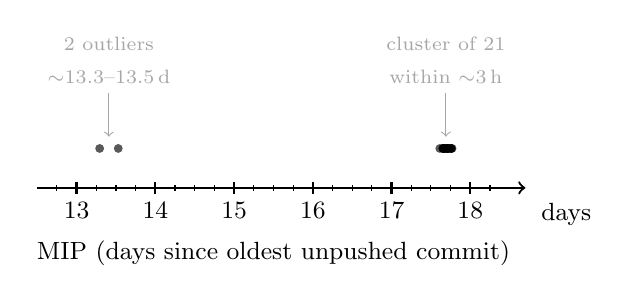
\begin{tikzpicture}[xscale=1.0]
  % Axis line from 12.5d to 18.5d
  \draw[->, thick] (12.5, 0) -- (18.7, 0) node[below right=2pt] {\small days};
  % Major tick marks at 13..18 with labels
  \foreach \x in {13, 14, 15, 16, 17, 18} {
    \draw[thick] (\x, -0.08) -- (\x, 0.08) node[below=4pt] {\small \x};
  }
  % Minor tick marks every 0.25d
  \foreach \x in {12.75, 13.25, 13.5, 13.75, 14.25, 14.5, 14.75, 15.25, 15.5, 15.75, 16.25, 16.5, 16.75, 17.25, 17.5, 17.75, 18.25} {
    \draw (\x, -0.04) -- (\x, 0.04);
  }
  % MIP values (days), 23 points
  \foreach \x in {13.2928, 13.5289, 17.6130, 17.6514, 17.6540, 17.6563, 17.6572, 17.6600, 17.6634, 17.6643, 17.6650, 17.6717, 17.6906, 17.7041, 17.7067, 17.7086, 17.7109, 17.7196, 17.7257, 17.7516, 17.7544, 17.7608, 17.7681} {
    \fill[black, opacity=0.65] (\x, 0.5) circle (1.6pt);
  }
  % Annotation arrows / labels
  \draw[<-, gray!70, thin] (13.41, 0.65) -- (13.41, 1.2) node[above, align=center] {\scriptsize 2 outliers\\\scriptsize $\sim$13.3--13.5\,d};
  \draw[<-, gray!70, thin] (17.69, 0.65) -- (17.69, 1.2) node[above, align=center] {\scriptsize cluster of 21\\\scriptsize within $\sim$3\,h};
  % x-axis label
  \node[below=10pt] at (15.5, -0.2) {\small MIP (days since oldest unpushed commit)};
\end{tikzpicture}
\caption{Strip plot of MIP values for the 23 repositories ahead of upstream at the baseline scan ($N=23$). Twenty-one repositories cluster within a $\sim$3-hour window near $17.7$ days---the bulk-event signature consistent with a single portfolio-wide directory restructure on 19 April 2026 that was never propagated. The two outliers near $13.3$--$13.5$ days correspond to commits made before the bulk operation that were also still unpushed. A post-intervention scan (after the operator pushed all 23) recorded zero repositories above the leakage threshold.}
\label{fig:mip-stripplot}
\end{figure}

A second finding tightens the implication for tooling (Section~6.2). Of 54 repositories that received agent touches in the scanned window, only 7 had a direct session whose working directory was the repository itself; the remaining 47 ($\approx$87\%) were touched exclusively from a parent directory via \texttt{cd <subrepo> \&\& git ...} and \texttt{git -C <subrepo>} chains. A na\"ive design that triggers ``intent-level CI/CD'' on session completion at the session's working directory would therefore miss the dominant pattern of agent-driven git activity in this portfolio. We treat this as evidence that agent-readability infrastructure must reason over command content, not just session metadata.

The companion observation is the inverse case: three repositories in the agent-touched cohort were not in the leakage set. Inspection shows they all sit in PR-routed workflows where push is part of the routine session loop or were freshly scaffolded with first-push as a setup step. The presence of these inverse cases bounds the metadatafication thesis: it does not predict that all agent-driven git activity becomes invisible, only that activity becomes invisible \textit{where attention has migrated away from git as a deliberate workflow surface}. After an operator-intervention push triggered manually upon discovering the baseline, a recovery scan recorded zero repositories above the leakage threshold, demonstrating that the breakdown is recoverable once the invisible state is rendered visible.

Finally, we note that the same breakdown-visibility pattern was independently observed in a sibling investigation of the IDE's session and worktree lifecycle on the same machine: stale worktrees from already-merged pull requests accumulated in the local Claude Code state until an external review surfaced them, with the IDE's own ``new PR'' picker exposing the head branches of those leftover worktrees as if they were active work.\footnote{This pattern is also documented in the Claude Code project itself, including issue \href{https://github.com/anthropics/claude-code/issues/26725}{\#26725 ``Stale worktrees are never cleaned up''} and \href{https://github.com/anthropics/claude-code/issues/43730}{\#43730 ``Worktree lifecycle: auto-cleanup or reuse across sessions''}, indicating the breakdown is not specific to one developer's environment but a structural feature of the current tooling. A May 2026 Claude Code release subsequently shipped two relevant fixes (``stale worktree cleanup race'' and ``improved stale agent worktree cleanup to remove worktrees whose PR was squash-merged''), reactively narrowing the breakdown after this paper's findings were drafted but without yet reorganising the design around the agent-readability principle of \S6.2. The third instance below has a parallel external precedent in the GitHub CLI: issue \href{https://github.com/cli/cli/issues/12980}{\#12980} (March 2026) reports that \texttt{gh pr merge -d} prints a ``Deleted remote branch'' confirmation while leaving the branch intact on the server, and issues \href{https://github.com/cli/cli/issues/9073}{\#9073} and \href{https://github.com/cli/cli/issues/11187}{\#11187} document the \texttt{--auto -d} non-deletion and the race-condition variants. The accumulating-stale-state failure mode is therefore independently exhibited across both agent-side and forge-side tooling.} The recovery action there---``Auto-archive on PR close''---is itself an opt-in setting, suggesting that the default tooling assumes the operator will manually inspect session lifecycle, exactly the assumption metadatafication predicts will fail.

A third instance, observed concurrently in the same session, sharpens the implication for tooling. The official command for merging a pull request and cleaning up its branches---\texttt{gh pr merge --delete-branch}---splits internally into a server-side merge call and a client-side cleanup that runs \texttt{git push origin --delete} and \texttt{git branch -D}. When the branch being deleted is held by a sibling git worktree (a common configuration when an agent has spawned isolated work environments under \texttt{.claude/worktrees/}), the cleanup step fails silently while the server-side merge succeeds. The operator and the agent both see the merge as complete; the orphaned remote branch becomes background metadata and accumulates. In our two-repository comparison, the same workflow command produced zero stale branches in the repository worked from the main checkout (this paper's own repository, nine pull requests across this session) and accumulated more than ten stale remote branches in a sibling repository where parallel-worktree usage was the default. The three instances together---push-leakage, worktree-leakage, and command-cleanup-leakage---show that metadatafication is not bound to a single metadata kind but to a class of operator--tool interactions in which the tool does not reason over the operator's full topology. We treat this as the most concrete demonstration available to date of \S6.2's claim that ``agent-readability infrastructure must reason over command content, not just session metadata''---in this case, over the operator's worktree topology as a precondition for safe cleanup.

We mention these adjacent cases briefly because a full treatment requires its own instruments; the structural identity of all three (push-leakage, worktree-leakage, and command-cleanup-leakage as distinct metadata layers exhibiting the same breakdown mechanism) is sufficient signal that the thesis generalizes beyond any single metadata kind.

\paragraph{The mirror direction: external metadata that never reaches the agent.}
The three instances above all describe metadata flowing \textit{from} the agent that fails to propagate to its destination. A symmetric failure runs in the opposite direction: metadata produced by external contributors that fails to propagate \textit{to} the agent's attention. A concrete observation in this study: an external user filed a bug report (with a verified patch) on the operator's open-source MCP server on 24 April 2026; the operator opened 27 pull requests in that repository over the next 13 days, none of which referenced or addressed the report; the bug was discovered and fixed only after an explicit \texttt{gh issue list} prompt on 7 May 2026. The agent's session-start routine included \texttt{git status} and \texttt{gh pr list} but not \texttt{gh issue list}; the operator's own dashboard, which already exposed dependency and CI signal, did not at the time surface external-contributor issues either. Both signals converged: external metadata (the bug report) failed to enter either the agent's automatic check-list or the operator's normal field of view, even as the agent and operator interacted with the same repository dozens of times during the gap.

The structural identity is exact: an attention budget that does not enumerate a queue lets the queue accumulate. The fix mirrors the agent-side fixes: surface the queue in the operator's normal field of view (the dashboard that this paper's reference implementation now exposes via a portfolio-wide external-contributor-issues panel) and provide a programmatic surface (an MCP tool) so that any agent session, regardless of routine memory, can query the queue inline rather than depending on the operator to prompt for it. Listing this fourth instance separately matters for the framework: metadatafication is not a one-directional phenomenon (agent\,$\to$\,world); it is a property of \textit{any} metadata layer that an attention budget fails to scan. The recommendation in §6.2 thus generalises: agent-readability infrastructure must reason over command content \textit{and} treat external-contributor signal as part of the same operator-attention queue that push events live in.

\subsection{Evaluation: The Context Attention Metric}

To evaluate whether the attention redistribution predicted by the framework (Section~4.1) is observable in practice, we define the \textit{Context Attention Metric} (CAM): the fraction of commits in a rolling window that modify at least one \textit{agent-era} context artifact. We then demonstrate its computability across 32 repositories and report initial signals.

We distinguish agent-era artifacts---files that exist specifically to instruct AI agents (AGENTS.md, CLAUDE.md, \texttt{.cursorrules}, \texttt{copilot-instructions.md}, structured specification files)---from legacy configuration (tsconfig.json, ESLint configs, CI workflows) that predates the agentic turn. Only the former directly evidence attention migration toward context engineering; the latter inflate the ratio without supporting the thesis.

\begin{equation}
\text{CAM} = \frac{|\{c \in C_{90} : c \text{ touches at least one agent-era artifact}\}|}{|C_{90}|}
\end{equation}

\noindent where $C_{90}$ is the set of commits in the most recent 90-day window. The metric can be computed from data Canary already collects (commit history via the GitHub API and file tree classification) without additional API calls.

To control for circularity (the author's portfolio is biased toward AI-assisted development), we measure CAM for both the portfolio and an external reference sample of 24 repositories spanning 7 programming ecosystems. The reference sample is explicitly split into \textit{AI-adjacent} projects (Vercel AI, LangChain, Anthropic Cookbook; $n=3$) and \textit{traditional} open-source projects with no inherent AI connection ($n=21$), the latter covering JavaScript/TypeScript (React, Next.js, TypeScript, Node.js, Svelte, Remix, Vite, Deno, shadcn/ui, Tailwind CSS), systems languages (Linux, Rust, Go, Docker, Prometheus), and Python/Java (CPython, Django, Flask, Spring Boot, Kafka). Repositories with fewer than 5 commits in the window are excluded ($n=9$).

\textbf{Results.} Table~\ref{tab:cam} summarizes CAM values for the 90-day window ending April 2026 across 32 included repositories.

\begin{table}[ht]
\centering
\small
\begin{tabularx}{\textwidth}{lrrrr}
\toprule
\textbf{Subgroup} & \textbf{$n$} & \textbf{w/ agent files} & \textbf{Mean CAM} & \textbf{Median CAM} \\
\midrule
User portfolio ($\geq$5 commits) & 8 & 2 (25\%) & 2.1\% & 0.0\% \\
Reference: AI-adjacent & 3 & 3 (100\%) & 2.5\% & 1.9\% \\
Reference: Traditional & 21 & 11 (52\%) & 0.8\% & 0.0\% \\
\midrule
Reference: All & 24 & 14 (58\%) & 1.0\% & 0.2\% \\
\bottomrule
\end{tabularx}
\caption{Context Attention Metric by subgroup ($n=32$, repos with $<5$ commits excluded). Agent-era files: AGENTS.md, CLAUDE.md, \texttt{.cursorrules}, \texttt{copilot-instructions.md}.}
\label{tab:cam}
\end{table}

Two findings stand out. First, \textit{adoption is governance-dependent}: 11 of 21 traditional repositories (52\%) contain agent-era files, but commit activity on them concentrates in developer-led projects---React (CLAUDE.md, CAM = 4.1\%), Next.js (AGENTS.md, CLAUDE.md, CAM = 2.0\%), TypeScript (AGENTS.md, copilot-instructions.md), Remix (AGENTS.md in multiple packages, CAM = 6.8\%), Deno (CLAUDE.md), Svelte (AGENTS.md), and Vite (copilot-instructions.md). Foundation-governed projects show a qualitatively different pattern: while three have adopted agent-era files---Prometheus (AGENTS.md, CLAUDE.md, CAM = 0.8\%), Django (copilot-instructions.md, CAM = 0.4\%), and Rust (rust-analyzer subproject, CAM $\approx$ 0.0\%)---the remaining eight (Linux, Kubernetes, CPython, Go, Node.js, Docker, Spring Boot, Kafka) show zero adoption. We classify projects as \textit{foundation-governed} if their primary governance authority is a non-profit foundation (Apache, CNCF, PSF, OpenJS, Rust Foundation, DSF) or they follow a formal proposal process (PEP, KEP, Go proposals); all others are \textit{developer-led} (full classification table in replication package). A Mann-Whitney U test confirms the difference: developer-led projects ($n=10$, mean CAM = 1.6\%) differ significantly from foundation-governed projects ($n=11$, mean CAM = 0.1\%) with $U=21.0$, $z=2.39$, $p=0.017$, rank-biserial $r=0.62$ (large effect). Bootstrap 95\% CIs are [0.4\%, 3.0\%] for developer-led and [0.0\%, 0.3\%] for foundation-governed.

Second, \textit{creation outpaces maintenance}: by file type, AGENTS.md appears in 10 repos, CLAUDE.md in 9, copilot-instructions.md in 4, and .cursor configurations in 3, yet median CAM across all reference repos is only 0.2\%. Agent-era files are proliferating but not yet intensively maintained---commit activity on them remains $<$1\% for most adopters. This is consistent with early Phase~2 of the metadatafication model and with the finding by \citet{gloaguen2026evaluatingagentsmd} that context file quality, not merely presence, determines agent effectiveness.

\subsubsection{Temporal Trajectory}

To approximate the longitudinal trend without waiting for quarterly data, we computed CAM across five overlapping windows (30, 60, 90, 180, and 365 days) for the same repository set. Table~\ref{tab:cam-temporal} reports subgroup means.

\begin{table}[ht]
\centering
\small
\begin{tabularx}{\textwidth}{lrrrrr}
\toprule
\textbf{Subgroup} & \textbf{30d} & \textbf{60d} & \textbf{90d} & \textbf{180d} & \textbf{365d} \\
\midrule
AI-adjacent ($n=3$) & 1.9\% & 2.6\% & 2.5\% & 2.3\% & 1.5\% \\
Traditional ($n=21$) & 1.3\% & 0.8\% & 0.8\% & 0.5\% & 0.4\% \\
All reference ($n=24$) & 1.3\% & 1.0\% & 1.0\% & 0.7\% & 0.5\% \\
\bottomrule
\end{tabularx}
\caption{Mean CAM by time window. Shorter windows capture more recent activity; longer windows dilute recent commits with older history.}
\label{tab:cam-temporal}
\end{table}

The monotonic increase from 365d to 30d in traditional OSS---0.4\% $\to$ 1.3\%, a 3$\times$ increase---indicates that context-file activity is \textit{accelerating}, not merely present. Per-repo trends reinforce this: TypeScript surged from 1.9\% (365d) to 11.1\% (30d), React from 0.7\% to 3.2\%, Svelte from 0.1\% to 1.3\%, and Deno from 0.2\% to 1.3\%. Most foundation-governed projects remain at 0.0\% across all windows (Linux, Kubernetes, CPython, Go, Node.js, Docker, Spring Boot, Kafka), though two foundation-governed adopters---Prometheus (0.3\% $\to$ 2.7\%) and Django (0.1\% $\to$ 1.3\%)---show the same accelerating pattern, suggesting that governance slows initial adoption but does not prevent intensification once it occurs. Because the windows overlap, these are not independent samples; however, they provide strong descriptive evidence that the trend direction is upward for adopting projects regardless of governance model.

\subsubsection{Diff Volume: CAM-LOC}

Commit count alone may overstate attention if context-file commits are trivially small (e.g., initial file creation). To control for this, we define a complementary metric:

\begin{equation}
\text{CAM-LOC} = \frac{\sum \text{lines changed in agent-era files}}{\sum \text{lines changed (all files)}} \quad \text{(90-day window)}
\end{equation}

\noindent Table~\ref{tab:cam-loc} compares CAM (commit-based) with CAM-LOC (diff-volume-based) for the 14 repositories that contain agent-era files.

\begin{table}[ht]
\centering
\small
\begin{tabularx}{\textwidth}{lrrrrr}
\toprule
\textbf{Repository} & \textbf{CAM} & \textbf{CAM-LOC} & \textbf{Agent LOC} & \textbf{Total LOC} & \textbf{Ratio} \\
\midrule
remix-run/remix & 2.0\% & 1.01\% & 893 & 88{,}375 & 0.51 \\
prometheus/prometheus & 3.0\% & 0.74\% & 410 & 55{,}404 & 0.25 \\
facebook/react & 4.1\% & 0.42\% & 305 & 72{,}025 & 0.10 \\
denoland/deno & 1.0\% & 0.23\% & 151 & 65{,}637 & 0.23 \\
django/django & 0.5\% & 0.11\% & 10 & 9{,}251 & 0.22 \\
sveltejs/svelte & 0.5\% & 0.05\% & 9 & 19{,}674 & 0.09 \\
vercel/next.js & 2.0\% & 0.04\% & 24 & 56{,}201 & 0.02 \\
microsoft/typescript & 1.3\% & 0.03\% & 59 & 170{,}348 & 0.03 \\
vercel/ai & 1.0\% & 0.02\% & 19 & 116{,}504 & 0.02 \\
\bottomrule
\end{tabularx}
\caption{CAM vs.\ CAM-LOC for repositories with agent-era file activity. The Ratio column = CAM-LOC / CAM; values $\ll 1$ indicate context-file commits are disproportionately small relative to their frequency.}
\label{tab:cam-loc}
\end{table}

The Ratio column reveals a bifurcation. Three projects invest substantial diff volume in context files: Remix (893 LOC across multiple package-level AGENTS.md files, Ratio = 0.51), Prometheus (410 LOC, primarily AGENTS.md creation, Ratio = 0.25), and React (305 LOC, primarily \texttt{compiler/CLAUDE.md}, Ratio = 0.10). These represent early \textit{refinement-phase} projects where context engineering is receiving genuine editorial attention. By contrast, most adopters show Ratios $\leq 0.03$---context-file commits exist but are trivially small, consistent with the creation-before-refinement pattern noted above.

The per-file breakdown corroborates this reading. React's \texttt{compiler/CLAUDE.md} accumulated 297 LOC of changes (+279 $-$18), indicating iterative refinement rather than one-time creation. Prometheus's AGENTS.md shows +352 $-$56, similarly suggesting active maintenance. In contrast, several repos show purely additive patterns (e.g., Django \texttt{copilot-instructions.md}: +10 $-$0; Svelte AGENTS.md: +9 $-$0), characteristic of initial creation without subsequent iteration.

Taken together, the temporal and diff-volume analyses strengthen the original CAM finding: agent-era files are not merely appearing but are receiving increasing commit attention (temporal CAM) and, in a subset of projects, substantive editorial investment (CAM-LOC). The ecosystem appears to be transitioning from Phase~2 (creation) toward Phase~3 (refinement) in the metadatafication model, with developer-led projects leading and foundation-governed projects yet to begin.

\subsubsection{Agent-Authored Commit Ratio}

CAM measures the ``input'' side of metadatafication---developer attention flowing \textit{toward} context engineering. But the thesis also predicts that Git records themselves become automatically generated. To measure this ``output'' side directly, we define the \textit{Agent-Authored Commit Ratio} (ACR): the fraction of commits whose metadata contains AI-agent co-authorship markers.

\begin{equation}
\text{ACR} = \frac{|\{c \in C_w : c \text{ has AI-agent marker}\}|}{|C_w|}
\end{equation}

\noindent We detect markers via \texttt{Co-authored-by} trailers referencing known AI tools (Claude, Copilot, Cursor, Devin) and bot-account login patterns. We separately classify traditional automation (Dependabot, Renovate, GitHub Actions) to distinguish pre-AI automation from agent authorship. Because many AI-assisted commits lack markers (Copilot and Cursor rarely annotate), ACR is a conservative lower bound: the true fraction of agent-influenced commits is higher.

\begin{table}[ht]
\centering
\small
\begin{tabularx}{\textwidth}{lrrrrrr}
\toprule
\textbf{Subgroup} & \textbf{$n$} & \textbf{30d ACR} & \textbf{90d ACR} & \textbf{365d ACR} & \textbf{90d Bot} & \textbf{90d Auto} \\
\midrule
User portfolio & 8 & 20.5\% & 20.9\% & 20.9\% & 3.6\% & 24.5\% \\
AI-adjacent & 3 & 3.8\% & 5.9\% & 11.0\% & 23.3\% & 29.1\% \\
Traditional & 21 & 6.4\% & 5.0\% & 4.3\% & 3.5\% & 8.5\% \\
\midrule
All reference & 24 & 6.1\% & 5.1\% & 5.2\% & 6.0\% & 11.1\% \\
\bottomrule
\end{tabularx}
\caption{Agent-Authored Commit Ratio (ACR) by subgroup and window. ``Bot'' = traditional automation (Dependabot, Renovate, etc.). ``Auto'' = AI + Bot combined. ACR is a lower bound due to unmarked AI-assisted commits.}
\label{tab:acr}
\end{table}

Three findings emerge. First, \textit{agent authorship is already substantial}: even as a lower bound, mean ACR for traditional OSS is 5.0\% (bootstrap 95\% CI: [1.2\%, 10.9\%]) at 90 days. Individual projects far exceed this---Deno (56.6\%), TypeScript (13.0\% at 90d, 33.3\% at 30d), Next.js (11.6\%), Tailwind CSS (6.6\%), and Vite (5.4\%). These are not peripheral projects; they are foundational infrastructure of the modern web ecosystem.

Second, \textit{agent authorship is accelerating in traditional OSS}: mean ACR rises from 4.3\% (365d) to 6.4\% (30d). TypeScript's surge from 7.4\% (365d) to 33.3\% (30d) is particularly striking. Claude dominates the detected markers (539 commits across all repos at 90d), followed by Copilot (35) and Cursor (12), though Copilot's true contribution is likely understated due to its inconsistent use of co-authorship markers.

Third, \textit{the governance divide persists}: developer-led projects (mean ACR = 10.0\%, CI: [2.8\%, 21.4\%]) significantly exceed foundation-governed projects (mean ACR = 0.3\%, CI: [0.1\%, 0.6\%]). A Mann-Whitney U test yields $U=21.0$, $z=2.39$, $p=0.017$, rank-biserial $r=0.62$ (large effect). Linux (0.0\%), Kubernetes (0.0\%), Django (0.0\%), and Spring Boot (0.0\%) show zero detected AI authorship, while Go (0.2\%), Rust (0.2\%), Docker (0.3\%), and CPython (0.6\%) show only trace amounts. Notably, Django's agent-era file (\texttt{copilot-instructions.md}) was created explicitly to \textit{discourage} automated AI reviews of pull requests---an instance of governance using the mechanism of context engineering to \textit{limit} rather than enable agent participation. Even among foundation-governed repos, sporadic agent-authored contributions appear (Apache Kafka 1.1\%, Prometheus 0.6\%, CPython 0.6\%)---agents submit patches to these projects regardless of project-level adoption, a pattern consistent with externally-driven agent use by individual contributors.

ACR provides the missing ``output'' evidence for metadatafication: Git commit records are not merely being consumed differently (CAM) but are being \textit{produced} by agents at scale. When over half of Deno's recent commits and a third of TypeScript's carry AI co-authorship markers---and these are conservative lower bounds---the characterization of Git as ``automatically-generated metadata'' is not aspirational but descriptive.

\subsubsection{Adoption Timeline}

To distinguish a sustained wave of adoption from legacy file presence, we traced the first commit date for each agent-era file across the 26 reference repositories. Figure~\ref{tab:adoption} shows the cumulative adoption curve.

\begin{table}[ht]
\centering
\small
\begin{tabularx}{\textwidth}{lrl}
\toprule
\textbf{Month} & \textbf{Cumulative} & \textbf{New adopters} \\
\midrule
2025-06 & 1/26 & TypeScript (copilot-instructions.md) \\
2025-07 & 3/26 & Vite, LangChain \\
2025-10 & 5/26 & Remix, Anthropic Cookbook \\
2025-11 & 6/26 & Deno \\
2026-01 & 9/26 & Next.js, Vercel AI, React \\
2026-03 & 13/26 & Rust, Django, Prometheus, shadcn/ui \\
2026-04 & 14/26 & Svelte \\
\bottomrule
\end{tabularx}
\caption{Cumulative adoption of agent-era files among 26 reference repositories. The rate accelerated sharply in Q1 2026.}
\label{tab:adoption}
\end{table}

The adoption curve is convex: 1 repo in the first 7 months (June--December 2025), then 8 repos in the next 4 months (January--April 2026). The earliest adopter was TypeScript's \texttt{copilot-instructions.md} (June 2025); by file type, \texttt{copilot-instructions.md} appeared first (2025-06), followed by CLAUDE.md (2025-07), AGENTS.md (2025-09), and \texttt{.cursor} configurations (2026-01)---a progression from tool-specific to tool-agnostic formats. The 12 non-adopting repos are exclusively foundation-governed (Linux, Kubernetes, Go, CPython, Node.js, Docker, Spring Boot, Kafka) or projects with low recent activity (Flask, Tailwind CSS), reinforcing the governance moderation finding.

\section{Implications}

\subsection{For Developer Education}

If Git becomes infrastructure metadata, teaching Git mechanics to beginning developers becomes analogous to teaching assembly language: valuable for deep understanding but no longer a prerequisite for productive work. Educational curricula should shift emphasis toward specification writing, context engineering, outcome verification, and agent orchestration. This does not mean Git knowledge becomes worthless---DNS expertise remains valuable for network engineers---but it becomes a \textit{specialization} rather than a \textit{universal prerequisite}.

\subsection{For Tooling}

Current development tools assume that humans read and write code. The metadatafication thesis implies a need for tools designed around the assumption that agents read and write code, and humans read and write \textit{intent}: agent-native VCS \citep{atomic2026, cohen2026manyana}, intent-level CI/CD triggered by agent session completion rather than \texttt{git push}, and context-first IDEs organized around specifications and agent configuration rather than file trees.

The agent-session-completion trigger is concretely demonstrated in Section~5.4. The push-leakage instrument enumerates repositories whose unpushed work would be invisible to a tool watching only the session's working directory; the parent-cwd opacity finding (87\% of agent-touched repositories in the reported portfolio were touched only via \texttt{cd \textless subrepo\textgreater\ \&\& git ...} chains) shows that any such trigger must reason over the bash command content rather than the session metadata alone. The same vignette identifies two adjacent failure modes---worktree-leakage (stale worktrees from already-merged pull requests) and command-cleanup-leakage (silent partial failure of \texttt{gh pr merge --delete-branch} when sibling worktrees hold the branch)---both of which the same recommendation addresses: tools that do not reason over the operator's full topology will produce invisible accumulating metadata, and the recovery affordance must be opt-out by default rather than opt-in.

A nascent class of worktree-aware tooling already moves in this direction. Worktrunk\footnote{\url{https://worktrunk.dev/}}, CodeRabbit's \texttt{git-worktree-runner}\footnote{\url{https://github.com/coderabbitai/git-worktree-runner}}, the \texttt{git-worktree-toolbox} MCP server\footnote{\url{https://github.com/ben-rogerson/git-worktree-toolbox}}, and Cursor's Agents Window (April 2026) all treat parallel worktrees as first-class objects in agent workflows, providing automation hooks and lifecycle commands that the bare \texttt{git worktree} interface lacks. They are reactive responses to the same operator-budget pressures that produce metadatafication; whether they evolve into the agent-readability infrastructure the framework predicts---reasoning over command content, intent-aware merges, opt-out defaults---remains an open empirical question, but the direction of movement matches the framework's prediction.

The metric naming in Section~5.4 is a deliberate choice rather than a borrowed term. Survey on 7 May 2026 turned up no academic or commercial usage of ``working-tree staleness'' or ``uncommitted period'' as a developer-productivity metric, despite extensive prior work on developer-productivity frameworks (DORA, SPACE, DevEx; consolidated more recently into the DX Core 4 model with four dimensions of speed, effectiveness, quality, and business impact). MIP, APL, PLR, and UCP fit naturally as a fifth dimension---\textit{operator--tool topology hygiene}---that none of those frameworks measure today, because the operator--tool relationships they encode predate AI agents as primary commit authors. Position the four metrics accordingly: not as a replacement for DORA-style flow metrics but as a layer that becomes legible only once a substantial fraction of git activity is agent-driven.

\subsection{For Ecosystem Governance}

The shift from app stores to capability marketplaces raises governance questions: How are MCP capability providers vetted? What prevents malicious capabilities from being composed into user-facing applications? When an agent chains multiple capabilities, who is responsible for emergent behaviors? What economic model sustains a marketplace where the ``app'' is generated on the fly? These questions remain open and represent significant opportunities for both research and entrepreneurship.

\section{Counterarguments and Limitations}

\textbf{Non-determinism undermines prompt-as-source.} LLMs produce varying outputs from identical inputs \citep{hn2026provenance}, making pure intent-based versioning unreliable. This is why we argue for metadatafication (Git persists as automatically-generated metadata) rather than replacement. The non-determinism argument \textit{strengthens} the case for retaining version control records---but as metadata, not as primary developer artifacts. A deeper structural analysis reveals a \emph{verification paradox}: even if representation-level systems resolve non-determinism at the generation stage, formal verification still requires projection to code form, reintroducing the formal-language constraint at the verification stage~\citep{zgap2026chomsky}. This paradox reinforces our thesis: version control records persist precisely because verification cannot be fully abstracted away.

\textbf{Regulatory and compliance pressures.} Standards such as SLSA (Supply-chain Levels for Software Artifacts) and regulations including HIPAA, SOX, and the EU AI Act increasingly require auditable provenance trails for software artifacts. In an agentic regime, these requirements make Git records \textit{more} important for compliance, not less---but the audience shifts from developers to auditors, automated compliance tools, and legal review. This is consistent with metadatafication: the records persist and gain regulatory significance, while ceasing to be a site of daily developer attention.

\textbf{Edge cases require deployment history.} \citet{kirsch2026flawed} argues that edge cases emerge only through deployed use, and regenerating software resets this discovery. This is compatible with metadatafication: deployment history is precisely the kind of automatically-generated metadata that persists without direct developer interaction.

\textbf{Critical systems require formal verification.} We do not claim metadatafication applies uniformly. Safety-critical domains will continue to require human-auditable version control. Metadatafication describes a trajectory for the majority of software development, not a universal law.

\textbf{Network effects protect Git.} Git's dominance is sustained by ecosystem integration as much as technical merit. This is a claim about \textit{speed} of transition, not \textit{direction}.

\textbf{Malleable vs.\ ephemeral.} \citet{kirsch2026flawed} proposes ``malleable software'' as a more realistic alternative to ephemeral software. We view this as compatible: malleable software still shifts developer attention from code manipulation to intent specification.

\textbf{Context files can hurt agent performance.} \citet{gloaguen2026evaluatingagentsmd} find that LLM-generated AGENTS.md files reduce task success rates by up to 3\% and increase inference costs by over 20\%. This is an important finding that we do not dismiss. However, it does not undermine the metadatafication thesis---it constrains it. The finding shows that \textit{quality} of context artifacts matters more than their mere presence, and that the convention is not yet mature. This parallels early-stage patterns in other metadatafied technologies: misconfigured DNS records caused more failures than absent ones, but the solution was better configuration standards, not abandoning DNS. Our CAM data corroborate this reading: context files are proliferating (52\% adoption among traditional OSS) but are not yet intensively maintained (median CAM $<$ 1\%), suggesting the ecosystem is in the \textit{creation} phase before the \textit{refinement} phase that would produce performance gains.

\subsection{Threats to Validity}
\label{sec:tov}

\textbf{Construct validity.} CAM and ACR are proxy metrics for ``attention migration'' and ``automated record generation,'' respectively. CAM measures commit frequency touching agent-era files, not the cognitive attention developers invest; a developer may spend hours crafting an AGENTS.md file in a single commit, or may auto-generate it in seconds. CAM-LOC partially mitigates this by measuring diff volume, but neither metric captures time spent or cognitive effort. ACR relies on co-authorship markers, which are voluntarily applied and inconsistently adopted across tools. Copilot and Cursor rarely annotate commits, so ACR systematically undercounts agent involvement. We frame ACR as a conservative lower bound, but the magnitude of undercounting is unknown---the true agent-authored fraction could be substantially higher. Additionally, ``attention migration'' implies a zero-sum shift \textit{away from} code inspection, but our metrics only measure the \textit{toward context} direction; we present no direct evidence that developers are spending less time reading diffs or reviewing code.

\textbf{Internal validity.} The reference repository sample was selected purposively, not randomly. We chose well-known projects across 7 ecosystems to maximize diversity, but the selection is vulnerable to post-hoc bias: we may have unconsciously included projects known to have adopted agent-era files. The governance classification (developer-led vs.\ foundation-governed) is operationalized based on whether the project's primary governance authority is a non-profit foundation or it follows a formal proposal process (Section~5.4). While this criterion is more objectively verifiable than ad-hoc assignment, edge cases exist (e.g., corporate-backed projects with informal but gatekept review processes), and independent validation of the classification was not performed. The temporal CAM analysis uses overlapping windows (30d $\subset$ 60d $\subset$ 90d $\subset$ 180d $\subset$ 365d), so the observed ``acceleration'' could reflect a small number of recent file-creation events amplified in shorter windows rather than a sustained trend. Both Mann-Whitney U tests (CAM and ACR) reach significance at $p=0.017$, but with $n=21$ the tests have limited power, and the result is sensitive to governance classification choices (reclassifying two repositories shifted the ACR result from $p=0.060$ to $p=0.017$).

\textbf{External validity.} The sample of 26 reference repositories, while spanning 7 ecosystems, is small and skewed toward popular, English-language open-source projects. Adoption patterns may differ substantially in enterprise codebases, non-English developer communities, or smaller projects. The user portfolio ($n=8$) introduces circularity: the author uses Claude Code, which encourages CLAUDE.md creation. We control for this by reporting user and reference results separately and grounding our claims primarily in the reference sample. The ACR tool distribution (Claude: 539, Copilot: 35, Cursor: 12) reflects the current state of marker adoption, not the true market share of AI coding tools; conclusions about which tools drive metadatafication should be drawn cautiously.

\textbf{Reliability.} All experiments query the GitHub API at a specific point in time (April 2026). Results are inherently non-reproducible in the strict sense: re-running the scripts will produce different numbers as new commits accumulate and repositories evolve. We mitigate this by archiving raw JSON results alongside the scripts in a replication package committed to the artifact repository at the submission revision. The bootstrap confidence intervals provide a measure of sampling uncertainty but do not account for temporal instability of the underlying data.

\textbf{Single-operator scope is by design, not omission.} The case study in Section~\ref{sec:vignette} is drawn from one operator's portfolio. We treat this as the appropriate scope for the present contribution and not a limitation to apologise for. The framework-level claim is that a measurable instrument distinguishes bulk-operator breakdown from independent slippage; demonstrating that on one well-instrumented operator is sufficient to establish the instrument. The prevalence question (do other operators exhibit the same breakdown shape?) is a follow-up empirical study, complementary in scale and intent to \citet{li2025rise}'s 456k-PR macro-quantitative corpus rather than competing with it. Three concrete biases remain, and we name them. (i) Threshold choices (the 7-day MIP cutoff for the leakage classifier; the 30-day window for the recent-issues digest; the $\sim$3-hour spread used to characterise ``cluster'') are presented descriptively, not subjected to formal sensitivity analysis. The qualitative finding (degenerate MIP cluster + two earlier outliers) is robust to threshold variation in the ranges we explored, but a multi-operator follow-up would benefit from pre-registered thresholds. (ii) The researcher and the subject are the same person, with the author's thesis-confirmation incentive. We mitigate by reporting inverse cases (three agent-touched repositories not in the leakage set, including this paper's own repository), and by citing external corroboration: Claude Code project issues \href{https://github.com/anthropics/claude-code/issues/26725}{\#26725} and \href{https://github.com/anthropics/claude-code/issues/43730}{\#43730} document the worktree-leakage pattern independently of this study, and GitHub CLI \href{https://github.com/cli/cli/issues/12980}{\#12980} documents the command-cleanup-leakage pattern in the maintainers' own bug tracker. (iii) The portfolio composition (a research-heavy single-developer set) is unrepresentative of enterprise practice; we expect the bulk-event signature to be sharper in such a portfolio than in a typical team setting, and acknowledge that scaling the case to a team context likely smooths the cluster shape.

\textbf{Local-instrument reproducibility differs from GitHub-API reproducibility.} The push-leakage instrument operates on local filesystem state (git ahead/behind/dirty) and on Claude Code session transcripts under \texttt{\textasciitilde/.claude/projects/}, neither of which is queryable through any third-party API. A reader who clones the artifact will see different numbers because their machine has different repositories, different transcripts, and a different attention history. Reproducibility here is structural---the instrument is reproducible (anyone can run it on their portfolio) but the values it returns are inherently personal. We treat this as a feature rather than a bug: the breakdown phenomenon the paper documents is itself a per-operator signal, and the instrument honours that. The archived vignette dataset (Zenodo deposit cited above) preserves the specific numbers the paper claims, frozen at the time of writing, for citation purposes; live runs are intended to surface the reader's own portfolio rather than reproduce the author's.

\section{Conclusion}

Git is not dying. It is becoming invisible.

The twenty-year trajectory of version control follows a pattern repeated across computing infrastructure: technologies that once demanded direct human expertise become automatically-operated background layers. EXIF, DNS, TCP/IP, file systems, and compiler optimization all traversed this path. Git is next.

The implications extend beyond version control. As AI agents become the primary authors of code, the entire software ecosystem---from how code is reviewed, to how software is distributed, to how capabilities are reused---is restructuring around a new division of labor. Developers specify intent and verify outcomes; agents handle implementation and tooling. Git records persist as infrastructure metadata: automatically generated, systematically stored, and consulted only under exceptional circumstances.

The community that thrives in this transition will not be the one with the deepest Git expertise. It will be the one that best answers a different question: \textit{how do we structure our knowledge so that agents can act on it effectively?} The next GitHub is not a better Git forge. It is a capability marketplace---and the race to build it has already begun.

\bibliographystyle{plainnat}
\bibliography{references}

\end{document}
